\chapter{Methodology}
\begin{quote}
What I cannot create, I do not understand.
\end{quote}
\hfill --- Richard Feynman 
\vspace{0.5in}

The main contributions of this thesis are new models of pose which allow us to 
incorporate new image representations.  In this part we show empirically that the new 
representations are worthwhile by comparing them to state-of-the-art methods on 
competitive benchmark datasets.  Furthermore, we also analyze the trade-offs of 
the different models and the features' effectiveness.

\section{Datasets}\label{sec:datasets}
\begin{figure}[tb!]
\begin{center}
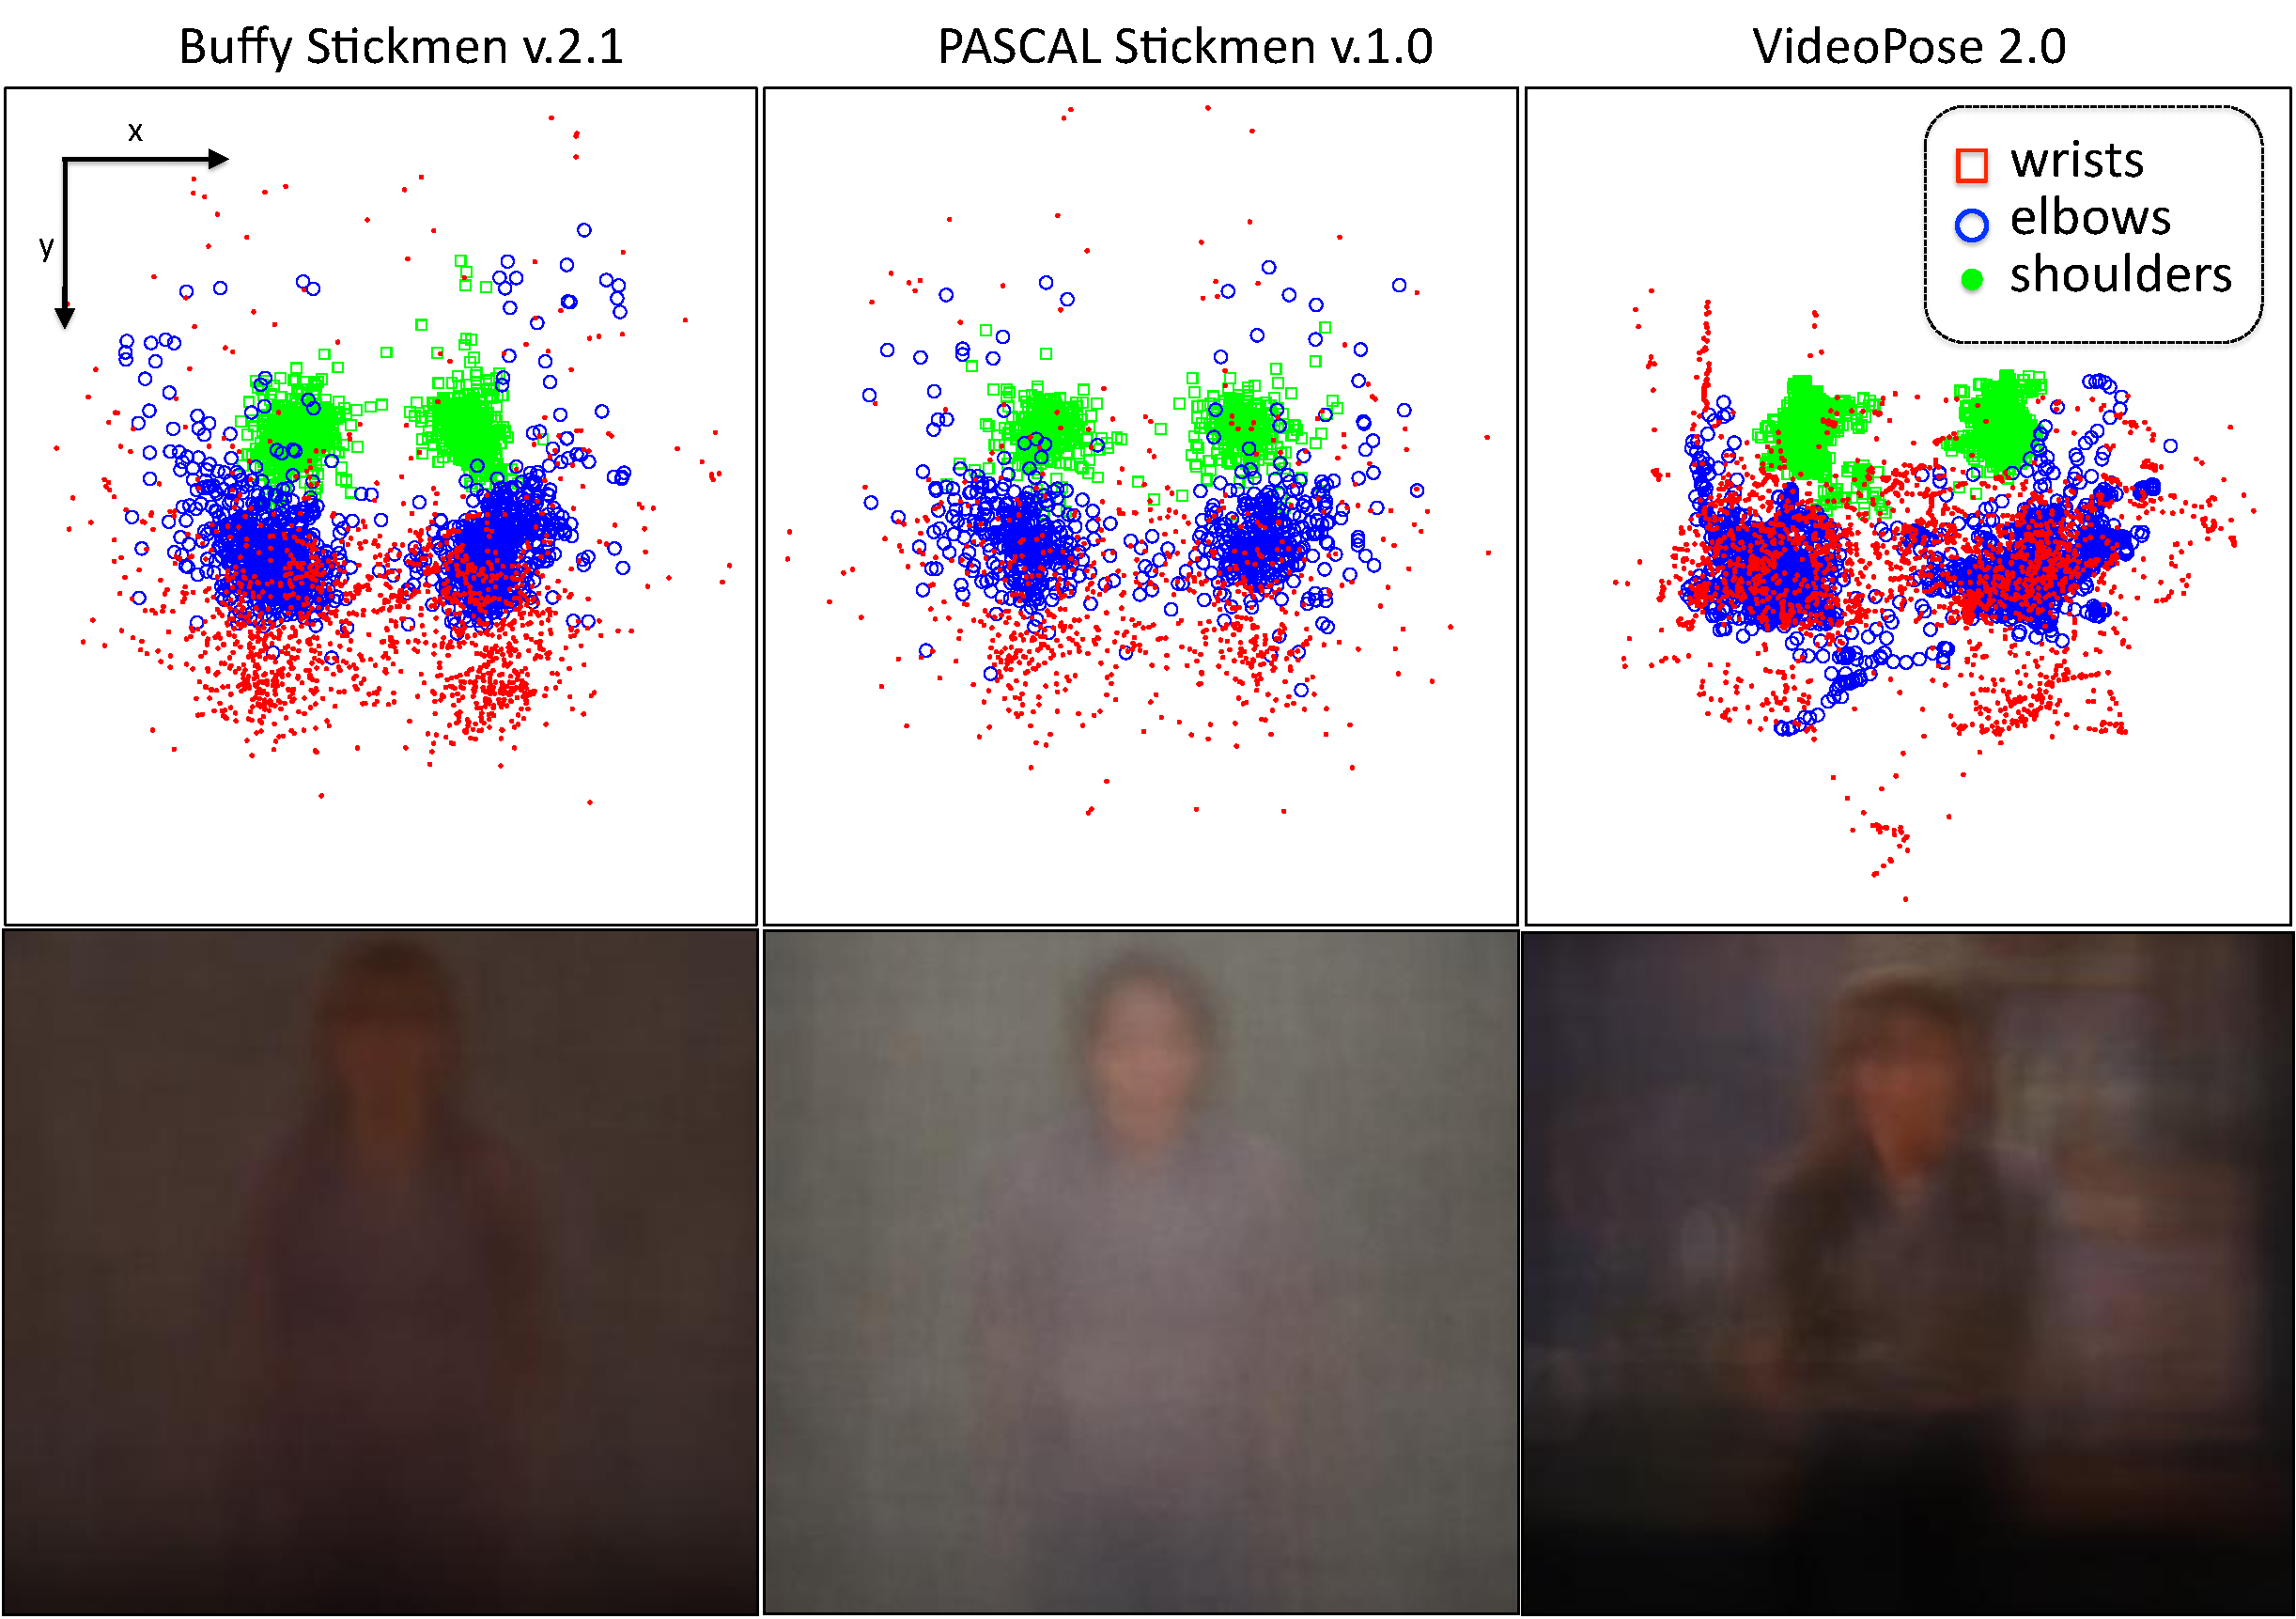
\includegraphics[width=1.05\textwidth]{figs/dataset-scatterplots.pdf}
\caption[Dataset joint scatterplots and pixel averages.]{Dataset joint 
scatterplots and pixel averages.  Here we show the spatial distribution of 
wrist, elbow and shoulder joints for our three datasets, both training and 
test, top row.  Bottom row, the average images from each of the datasets, with 
manually enhanced brightness and contrast for better visualization.}
\label{fig:dataset-scatterplots}
\end{center}
\end{figure}



We evaluate our methods on four publicly available datasets; two developed through the course of this research.

\subsection{Buffy Stickmen}
This dataset was first introduced in \citet{ferrari08}.  We use version 2.1 in 
our experiments, consisting of 748 frames from the TV show Buffy the Vampire 
Slayer, from episodes 2, 4, 5 and 6 from season 5.  The standard protocol is to 
test on a given set of 235 frames that were correctly localized by an upper 
body detector in~\citet{ferrari08}---within 50\% overlap with the groundtruth.  
For training images where an upper body detector did not detect a person for 
which we have annotated limbs, we loosely annotated the upper body manually to 
simulate test time behavior.
  

\subsection{PASCAL Stickmen}  This dataset was first introduced by 
\citet{eichner09} and contains 360 examples (version 1.0) obtained from amateur 
photographs culled from the PASCAL VOC 2008 challenge~\citep{voc09}.  This is 
purely a test dataset; the standard protocol is to train a model on Buffy 
images and test on PASCAL Stickmen. We follow this protocol for CPS, and for 
LLPS we train using the larger MoviePose dataset, discussed next.

\subsection{MoviePose}
Large datasets are crucial when we want to learn rich models of realistic pose.
The Buffy and PASCAL Stickmen datasets contain only a few hundred examples for 
training pose estimation models.  Other datasets exist with a few thousand 
images, but are lacking in certain ways. The H3D \citep{poselets} and PASCAL 
VOC \citep{voc09} datasets have thousands of images of people, but most are of 
insufficient resolution, significantly non-frontal or occluded.  The UIUC 
Sports dataset \citep{wang2011} has 1299 images but consists of a skewed 
distribution of canonical sports poses, \eg croquet, bike riding, badminton.  

Due to these shortcomings, we collected a $5003$ image dataset automatically 
from popular Hollywood movies, which we dub MoviePose.  The images were 
obtained by running a state-of-the-art person detector~\citep{poselets} on 
every tenth frame of $30$ movies, see \figref{movielist}.  People detected with 
high confidence were then sent to the crowdsourcing marketplace Amazon 
Mechanical Turk to obtain groundtruth labeling.  Each image was annotated by 
five Turk users for $\$0.01$ each to label 10 upperbody joints.  The median 
labeling was taken in each image to be robust to outlier annotation.  Finally, 
images were rejected manually by us if the person was occluded or severely 
non-frontal.  We set aside $20\%$ ($1016$ images) of the data for testing.

\begin{figure}[tb]
\begin{center}
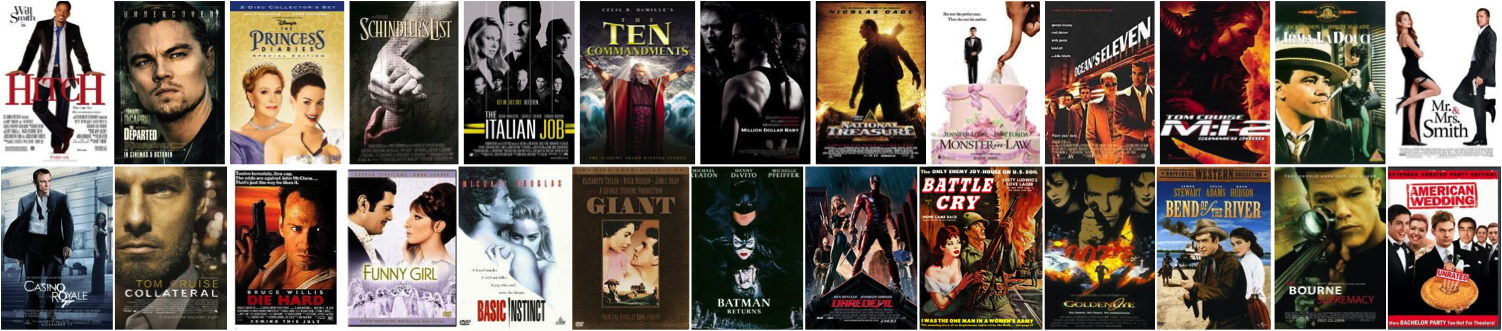
\includegraphics[width=1.00\textwidth]{figs/movie-list.png}
\caption[List of MoviePose movies]{A sampling of the 30 movies used in 
MoviePose.  The full list: {\em 12 O'Clock High, 2 Fast 2 Furious, Along Came 
Polly, American Wedding Unrated, Basic Instinct, Batman Returns, Battle Cry, 
Bend Of The River, Bourne Supremacy, Casino Royale, Collateral, Daredevil, 
Diehard 2, Flight Plan, Funny Girl, Giant Side, Goldeneye, Hitch, Irma La 
Douce, Italian Job, Million Dollar Baby, Monster In Law, Mr. \& Mrs.  Smith, 
National Treasure, Ocean's Eleven, Princess Diaries, Schindler's List, Ten 
Commandments, The Departed.}} \label{fig:movielist}
\end{center}
\end{figure}



\subsection{VideoPose}

We also apply our methods to a video dataset, which we collected ourselves: 
VideoPose 2.0.  Clips in the dataset were hand-selected (before developing our 
algorithm) to highlight natural settings where state-of-the-art methods fail: a 
highly varied (yet realistic) range of poses, rapid gesticulation, and a 
significant portion of frames (30\%) with foreshortened lower arms.  The 
dataset consists of 44 short clips, each 2-3 seconds in length, with a total of 
1,286 frames.  We use 26 clips for training, recycle 1 training clip for a 
development set, and use 18 for testing.  As in the Buffy and PASCAL datasets, 
we fix global scale and translation of the person---in this case by manual 
annotation.


\subsection{Discussion}  The datasets Buffy, Pascal, MoviePose and VideoPose 
have different biases, as can be seen in~\figref{dataset-scatterplots}.  First, 
note the distributions of joint locations.  The least varied is Buffy, followed 
by Pascal, MoviePose and then VideoPose.    In VideoPose in particular, the 
wrist locations have much more spread, and often lie on top of elbows, 
indicating more foreshortening in this dataset.  The hands are often raised up, 
gesticulating.  MoviePose has 5 to 10 times more exmaples than the other 
datasets.

Both Buffy and Pascal were collected with the 2D pictorial structure model in 
mind, where frames could be plucked individually to satisfy some of the 
2D-based assumptions of the model.  In the VideoPose dataset, we collected 
clips only based on duration, scale and viewpoint of the person.  MoviePose 
frames were selected automatically via a person detector.  Note that Buffy and 
Pascal both have less than 20 examples with elbows raised above shoulders, 
whereas VideoPose has none---this is an unusual pose for sitcoms and amateur 
photographs.

Second, observe the average images of these datasets in 
\figreff{dataset-scatterplots}{bottom}.  We can see plain biases---Buffy and 
VideoPose are darker (being primarily interior settings), the Buffy dataset is 
primarily female, and VideoPose has fewer unique background settings (the 
Friends' apartment, coffee shop, etcetera) which bias the average image.  
MoviePose has a significantly smoother average image than the rest, as it 
contains $5$ to $10$ times more data.


\section{Evaluation Measures}

Based on \probref{pose}, we wish to measure how well we recover ``line segments 
describing the major anatomical parts''.  Ideally, we want to measure how often 
our guessed pose matches a groundtruth pose.  However, this is nearly 
impossible in practice, even on the training set. It is very difficult to 
achieve anything near pixel-level precision---in practice, 1 pixel is 
approximately the size of a person's pupil at the resolution we use.  This lack 
of precision is due to uncertainty in human labeling, fixed-length limb models 
(in the case of classical PS and CPS), and translation invariant features which 
cannot guide limbs to extremely precise fits.

We consider the following relaxed measures of performance:

\subsection{Root-Mean-Square Error (RMSE)}  Because our datasets can be scale 
normalized (to the precision of an upper-body detector or groundtruth torso), 
pixel distances are meaningful across examples, and semantically meaningful.  
As such, we could measure accuracy via root-mean-square error, \ie the average 
Euclidean distance between predicted joints and the groundtruth joints on the 
test set.  However, when a guess is incorrect, it can be arbitrarily far away 
from the groundtruth, and arbitrarily skew the RMSE.  


\begin{figure}[t]
\begin{center}
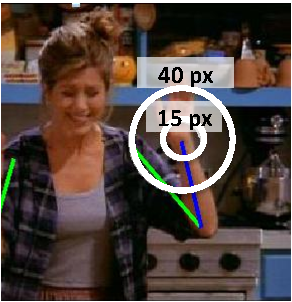
\includegraphics[width=0.42\textwidth]{figs/pixel-err-demo}
\caption[Joint error matching limits.]{Joint error matching limits.  We measure 
a range of pixel error distance thresholds to make a performance curve.}
\label{fig:pixel-err-demo}
\end{center}
\end{figure}


\subsection{Pixel error threshold}  In light of the outlier skewing problem of 
RMSE, we examine pixel accuracy at a range of thresholds.  At each threshold, 
we report the percent of test joint guesses that are within that Euclidean 
distance of the groundtruth, scaled by the size of the groundtruth torso.  We 
explore a range of thresholds, from very precise (the semantic distance of a 
average palm's width in pixels), to somewhat loose (the semantic distance of an 
average head's height in pixels).  This is illustrated in 
\figref{pixel-err-demo}.

The resulting performance curve gives us a good idea of accuracy at different 
operating points.  This is useful when assessing system for different 
applications. For example, it may be that for action recognition only a coarse 
notion of pose is required~\citep{wang2011}, but for automatic sign language 
understanding~\citep{buehler2009} we require near-certainty.

\subsection{Percentage of Correct Parts (PCP)}  Other works have proposed a 
measure Percentage of Correct Parts (PCP) that is a limb-based measure of 
correctness: a guess limb is correct if its endpoints lie within radii of the 
groundtruth endpoints, where the radii are half the length of the groundtruth 
limb~\citep{ferrari08,eichner09}.  The public implementation of this error 
measure \citep{eichner09} has some peculiarities: It uses a max-norm in a 
coordinate space aligned to the groundtruth limb, and allows arbitrary matching 
of endpoints (\eg, matching wrist to elbow is permissible).  This even allows 
correct matches that are perpendicular to the true limb, as long as the guess 
limb length is no longer than the true limb length and intersects the 
groundtruth limb at its midpoint.  

We prefer not to use PCP because (1) its criteria for a matched guess is too 
relaxed (2) is discontinuous (3) only considers one operating point instead of 
a range and (4) there are different interpretations of the metric leading to 
discrepancies in implementations (see the code release of \citet{eichner-tr}).  
However, for historical reasons, many works have reported results in terms of 
PCP, and here we do the same for compatibility.

\section{Competitor Methods}\label{sec:competition}

The field of 2D human pose estimation has exploded in the last 5 years.  The 
public datasets we report numbers on are highly competitive, with absolute 
performance rising each year since 2008.  We compare to several competing 
models.  Whenever possible, we report numbers in~\secref{results} from the 
publicly available implementations of competitors' code; these numbers are 
typically different than numbers reported in papers.  When public code is not 
available, we include PCP measures reported by the authors.

Note that the numbers reported here for our models are directly from our 
publicly available code, meaning any practitioner should be able to replicate 
results exactly.

\begin{itemize}
\item Mean pose baseline 

One reasonable sanity check is to compare against guessing the average pose in every te.  As 
can be seen in~\figref{dataset-scatterplots}, there is some centrality to the 
data, such that guessing the mean joint position will get some fraction of joints 
correct.  The mean pose is obtained by empirical averages of joint locations on 
the training sets; each joint estimated independently.

\item \citet{andriluka09} 

This is a classical dense PS method, as described in~\secref{ps}.  The unary 
limb detectors are trained Adaboost ensembles of Shape Context on top of Canny 
edges.  The pairwise potentials are standard unimodal geometric displacement 
costs, computed efficiently with distance transforms (\secref{dt}).

\item \citet{eichner09} 

This is a complex system built off of~\citet{devacrf}.  The initial unary term 
is linear filters on image edges.  It then iteratively re-parses using color 
estimated from the initial parse.  It also uses graphcut~\citep{boykov2001} to 
rule out some of the background clutter, and post-processing of probabilistic 
marginals to obtain final limb segments.

\item \citet{deva2011} 

This recent work uses HoG as its only image cue.  Like our models, it is 
trained jointly in a discriminative learning framework.  Contemporary with our 
proposed Stretchable Ensemble model, \citet{deva2011} also use joints as a 
basic unit of inference.  Their work focuses on modeling a several appearance 
modes for each part, which they treat as latent variables to be estimated 
during training.  \end{itemize}


\section{Implementation Details}\label{sec:impl-details}

Here we give various additional details about the implementation of our models. 
All the details of the various feature implementations are provided in 
\secref{features}. Code is available online at \begin{center} 
\url{http://vision.grasp.upenn.edu/video} \end{center}

\subsection{CPS}
\mypar{Coarse-to-Fine Cascade} While our fine-level state space has size $80 
\times 80 \times 24$, our first level cascade coarsens the state-space down to 
$10 \times 10 \times 12 = 1200$ states per part, which allows us to do 
exhaustive inference efficiently.  We train and prune with $\alpha = 0$, 
effectively learning to throw away half of the states at each stage.  In 
practice we adjust $\alpha$'s per part after a cascade stage is learned via 
cross-validation error, to prune as much as possible while retaining 95\% of 
the groundtruth validation hypotheses.

After pruning we double one of the dimensions (first angle, then the minimum of 
width or height) and repeat. In the coarse-to-fine stages we only use standard 
PS features.  HoG part detectors are run once over the original state space, 
and their outputs are resized to for features in coarser state spaces via 
max-pooling.  We also use the standard relative geometric cues as described in 
Sec.  4. We bin the values of each feature uniformly, which adds flexibility to 
the standard PS model—rather than learning a mean and covariance, multi-modal 
pairwise costs can be learned.

\mypar{Final stage} To obtain segments, we use NCut[19]. For the contour 
features we use 30 segments and for region moments – 125 segments.  As can be 
seen in~\secref{results}, the coarse-to-fine cascade leaves us with roughly 500 
hypotheses per part.  For these hypotheses, we generate all features mentioned 
in~\secref{features}.  For pairs of part hypotheses which are farther than 20\% 
of the image dimensions from the mean connection location, features are not 
evaluated and an additional feature indicating this is added to the feature 
set.  We concatenate all unary and pairwise features for part-pairs into a 
feature vector and learn boosting ensembles which give us our pairwise clique 
potentitals.  This method of learning clique potentials has several advantages 
over stochastic subgradient learning: it is faster to train, can determine 
better thresholds on features than uniform binning, and can combine different 
features in a tree to learn complex, non-linear interactions.  This approach is 
also a major selling point of~\citet{dtf2011}.

\subsection{Stretchable Ensembles}
Our chosen ensemble of tree models is a collection of six models that captures 
time persistence of each of the six joints, as well as left/right symmetric 
joint edges for left/right shoulder, elbows and wrists.  The decomposition is 
shown in~\figref{stretchable-overview}.  This covers all reasonable connections 
we could conceive of modeling, and allows us to incorporate all features 
mentioned in~\secref{features}.

As input to our method, we use potential shoulder and elbow locations generated 
by the coarse-to-fine cascade of CPS (\secref{CPS}), independently for each 
frame.  This typically yields 300-500 possible shoulder and elbow locations per 
image. For each of the 24 discrete elbow orientations predicted by CPS, we 
project possible wrist locations at 4 different lengths, chosen from the 5th, 
25th, 50th, and 75th lower arm length quantiles on the training set. We then 
take the top 500 wrist locations scored according to the foreground color 
features for each frame (\secref{features}). The result is a sparse set of 
locations for each joint with high recall.


\subsection{LLPS}
The MoviePose dataset contains $5003$ images, of which $1016$ are set aside for testing.  
This means we have $2\times 3987 = 7974$ half-image examples to learn our mode centers.  Based on cross-validation, we found $32$ modes to be most accurate in an end-to-end system.

